\documentclass[../../main.tex]{subfiles}
\graphicspath{{../../image/}{../../figure/}}
\begin{document}

\section{图像的生成对抗网络}\label{section:ch17-图像GAN}

GAN 的基本概念催生了大量的研究工作，涵盖了许多算法和众多应用，其中应用最广泛且成功的是图像生成。早期的 GAN 使用全连接网络作为生成器网络和判别器网络（参见第 10 章）。然而，使用卷积网络有许多好处，尤其是对于更高分辨率的图像而言。判别器网络将图像作为输入，并提供一个标量概率作为输出，因此使用标准的卷积网络非常合适（参见 10.5.3 小节）。生成器网络需要将低维潜空间映射成高分辨率图像，因此使用了基于转置卷积的网络，如图~\ref{fig:ch17-dcgan} 所示。

\begin{figure}[htbp]
\centering
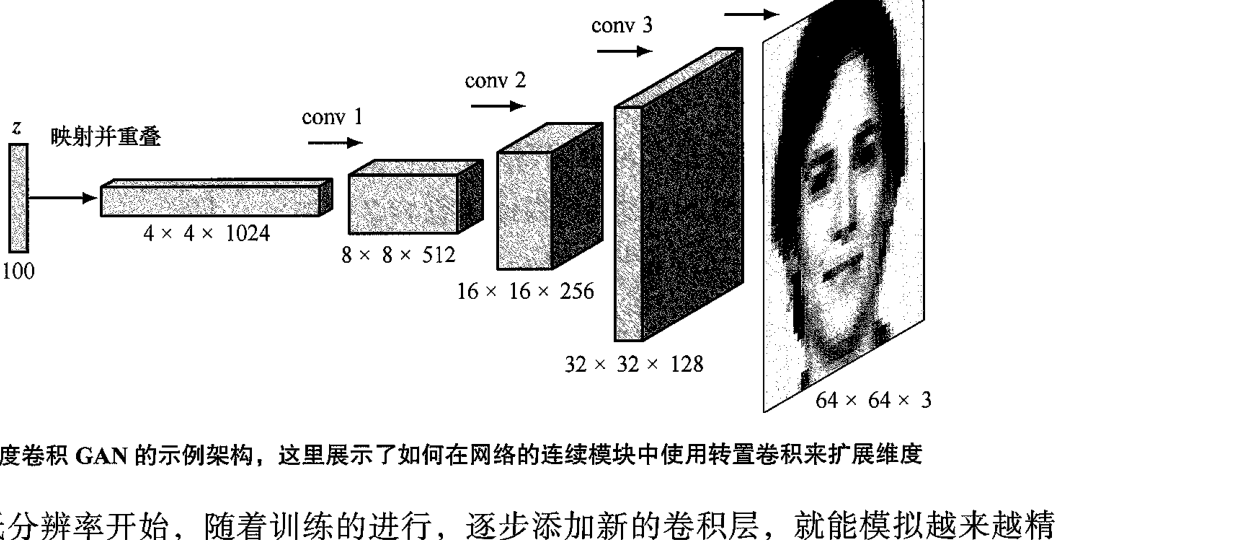
\includegraphics[width=0.85\textwidth]{ch17-fig488-dcgan.png}
\caption{深度卷积 GAN 的示例架构，这里展示了如何在网络的连续模块中使用转置卷积来扩展维度：从 $100$ 维潜向量出发，经 $4\times4\times1024$、$8\times8\times512$、$16\times16\times256$、$32\times32\times128$，最终得到 $64\times64\times3$ 的输出图像。}
\label{fig:ch17-dcgan}
\end{figure}

从低分辨率开始，随着训练的进行，逐步添加新的卷积层，就能模拟越来越精细的细节（Karras et al., 2017）。这种方法不仅加速了训练过程，而且能够从 $4\times4$ 大小的图像开始，最终合成 $1024\times1024$ 大小的高分辨率图像。

图~\ref{fig:ch17-biggan} 展示了用于类别条件图像生成的 GAN 模型---BigGAN，这是体现 GAN 架构的规模和复杂性的一个典型例子。BigGAN 的生成器网络拥有超过 $7000$ 万个参数，而拥有 $8800$ 万个参数的判别器网络具有类似的架构，不同之处在于判别器网络使用平均池化层（average pooling）来降低维度，而不是通过上采样（upsampling）来增加维度（Brock, Donahue, and Simonyan, 2018）。

\begin{figure}[htbp]
\centering
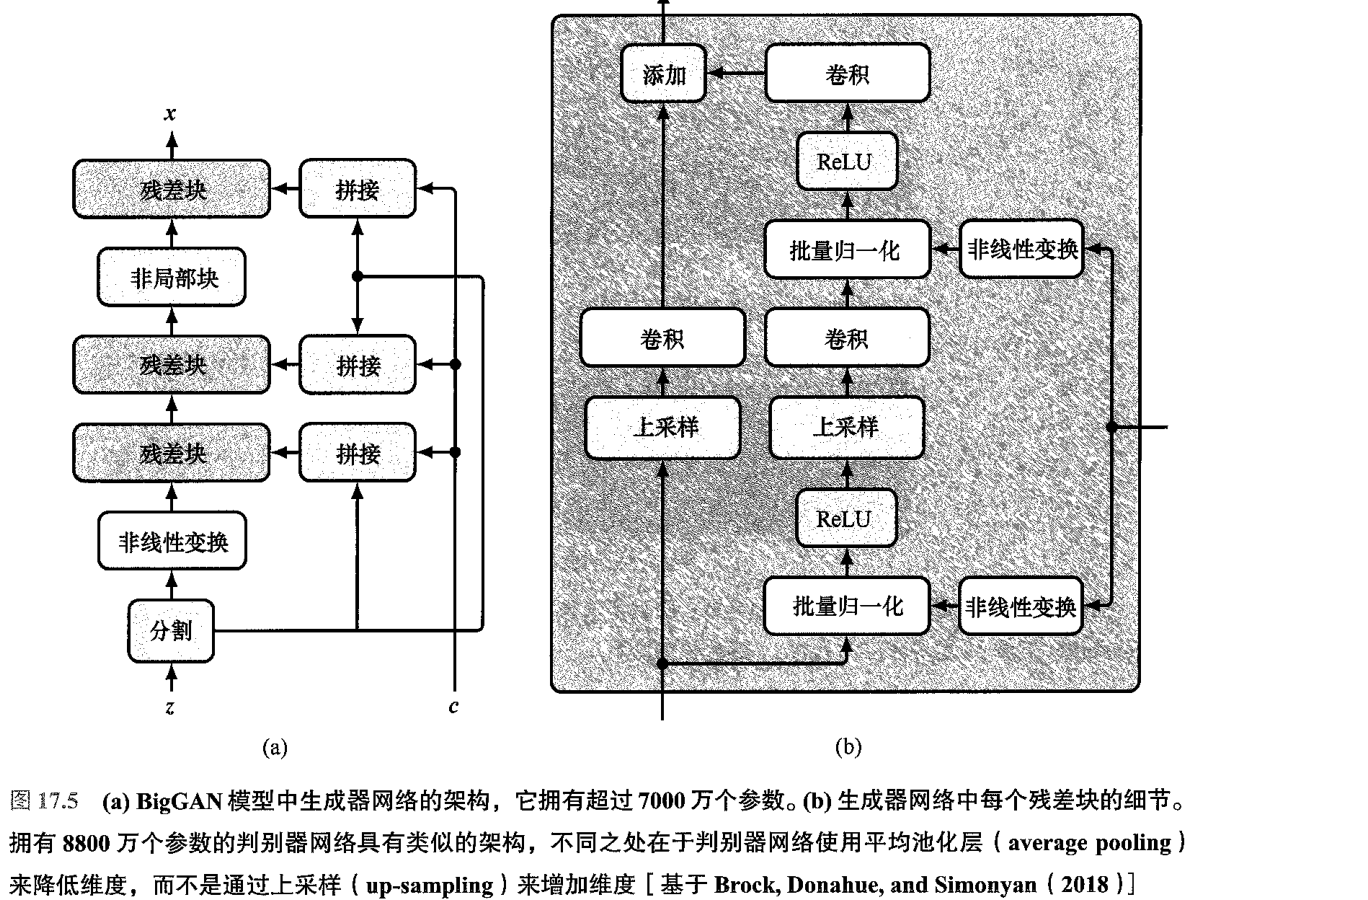
\includegraphics[width=0.9\textwidth]{ch17-fig489-biggan.png}
\caption{(a) BigGAN 模型中生成器网络的架构。(b) 生成器网络中每个残差块的细节，包含上采样、卷积、批量归一化、非线性变换、拼接与非局部块等组件。}
\label{fig:ch17-biggan}
\end{figure}

\subsection{CycleGAN}\label{subsection:ch17-cyclegan}

作为 GAN 多样性的一个例子，考虑一种称为 CycleGAN（Zhu et al., 2017）的 GAN 架构，我们将其作为示例以展示深度学习技术如何用于解决传统任务（如分类和密度估计）之外的不同类型的问题。考虑如下问题：如何将一张照片转换为同一场景下的莫奈风格的画作（或者反之）？

CycleGAN 的目标是学习两个双射（一对一映射），一个是从照片的域 $X$ 到莫奈风格画作的域 $Y$，另一个则相反。为了实现这一点，CycleGAN 利用了两个条件生成器（$g_X$ 和 $g_Y$）以及两个判别器（$d_X$ 和 $d_Y$）。生成器 $g_X(y,w_X)$ 以一幅画作 $y\in Y$ 为输入，并生成相应的合成照片，判别器 $d_X(x,\phi_X)$ 则区分合成照片和真实照片。类似地，生成器 $g_Y(x,w_Y)$ 以一张照片 $x\in X$ 为输入并生成一幅合成画作 $y$，判别器 $d_Y(y,\phi_Y)$ 则区分合成画作和真实画作。因此，对判别器 $d_X$ 的训练，需要结合 $g_X$ 生成的合成照片和真实照片来进行，而判别器 $d_Y$ 则是在 $g_Y$ 生成的合成画作和真实画作的组合上进行训练的。

\begin{figure}[htbp]
\centering
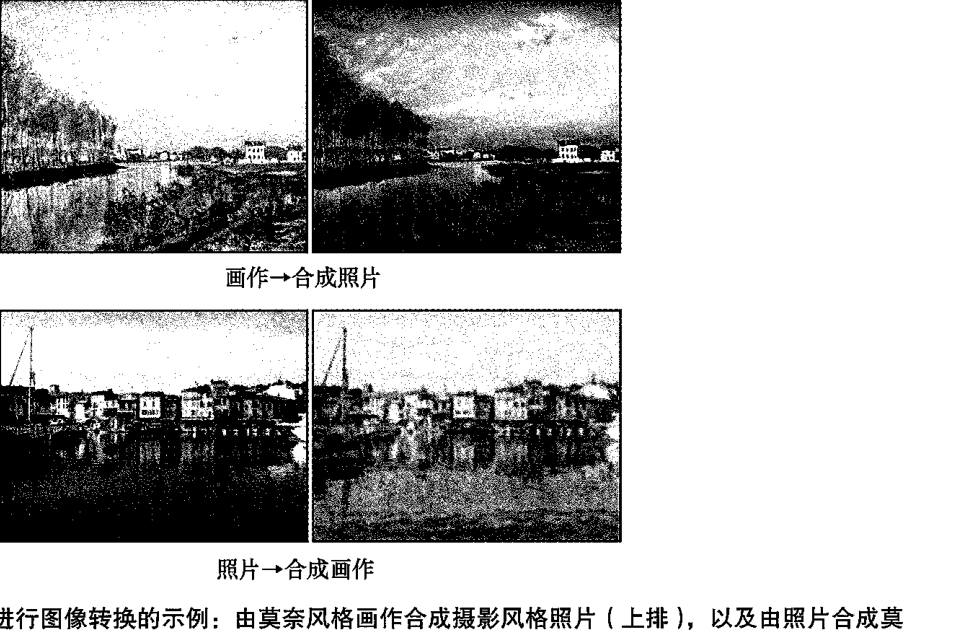
\includegraphics[width=0.85\textwidth]{ch17-fig490-cyclegan.png}
\caption{使用 CycleGAN 进行图像转换的示例：由莫奈风格画作合成摄影风格照片（上排），以及由照片合成莫奈风格画作（下排）（Zhu et al., 2017，经授权使用）。}
\label{fig:ch17-cyclegan}
\end{figure}

如果我们使用标准的 GAN 损失函数来训练这种架构，CycleGAN 就能学会生成逼真的合成画作和合成照片，但没有什么机制能确保生成的画作看起来像对应的照片，反之亦然。因此，我们在损失函数中引入了一个额外的术语，称为\textbf{循环一致性误差}（cycle consistency error）。它包含两项，其构建过程如图~\ref{fig:ch17-cycle} 所示。这一过程的目标是确保当一张照片先被转换成一幅画，再被转换回照片时，结果与原始照片接近，从而确保生成的画作保留了足以恢复原始照片的信息。类似地，当一幅画作先被转换成一张合成照片，再被转换回一幅画作时，结果也应该与原始画作接近。

\begin{figure}[htbp]
\centering
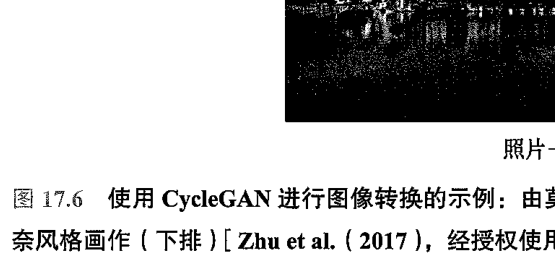
\includegraphics[width=0.8\textwidth]{ch17-fig491-cycle.png}
\caption{为示例照片 $x_n$ 计算循环一致性误差。首先使用生成器 $g_Y$ 将照片映射到画作域，然后将得到的向量映射回照片域，使用的是生成器 $g_X$。结果照片与原始照片 $x_n$ 之间的差异是由循环一致性误差贡献的。}
\label{fig:ch17-cycle}
\end{figure}

将这个理念应用到训练集中的所有照片和画作，就会得到形式如下的循环一致性误差：
\begin{align}
E(w_X,w_Y)=\frac{1}{N_X}\sum_{n=1}^{N_X}\big\|g_X\big(g_Y(x_n,w_Y),w_X\big)-x_n\big\|_1+\frac{1}{N_Y}\sum_{m=1}^{N_Y}\big\|g_Y\big(g_X(y_m,w_X),w_Y\big)-y_m\big\|_1
\label{align:ch17-cycle-loss}
\end{align}
其中 $\|\cdot\|_1$ 表示 $L_1$ 范数。将循环一致性误差添加到式~\eqref{align:ch17-egan} 定义的 GAN 损失函数中，便可得到总的损失函数：
\begin{align}
E_{\mathrm{total}}=E_{\mathrm{GAN}}(w_X,\phi_X)+E_{\mathrm{GAN}}(w_Y,\phi_Y)+\eta\, E(w_X,w_Y)
\label{align:ch17-total-loss}
\end{align}
其中系数 $\eta$ 决定了 GAN 误差和循环一致性误差的相对重要性。在计算一个图像和一幅画作的损失函数时，通过 CycleGAN 的信息流如图~\ref{fig:ch17-info-flow} 所示。

\begin{figure}[htbp]
\centering
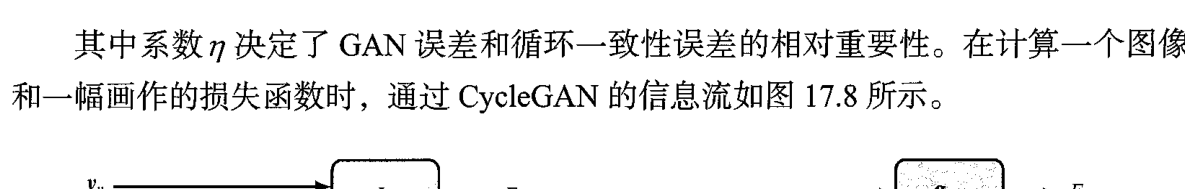
\includegraphics[width=0.85\textwidth]{ch17-fig492-info-flow.png}
\caption{通过 CycleGAN 的信息流。数据点 $x$ 和 $y$ 的总误差是其 $4$ 个组成部分误差的总和：两个方向的 GAN 误差与两个方向的循环一致性误差。}
\label{fig:ch17-info-flow}
\end{figure}

\end{document}